\documentclass[conference]{IEEEtran}
\IEEEoverridecommandlockouts
% The preceding line is only needed to identify funding in the first footnote. If that is unneeded, please comment it out.
\usepackage{cite}
\usepackage{amsmath,amssymb,amsfonts}
\usepackage{algorithmic}
\usepackage{graphicx}
\usepackage{textcomp}
\usepackage{xcolor}
\usepackage{verbatim}
%KHOA BEGIN
\usepackage{multirow}
\usepackage{array}
%KHOA END

\ifCLASSOPTIONcompsoc
    \usepackage[caption=false, font=normalsize, labelfont=sf, textfont=sf]{subfig}
\else
\usepackage[caption=false, font=footnotesize]{subfig}

\def\BibTeX{{\rm B\kern-.05em{\sc i\kern-.025em b}\kern-.08em
    T\kern-.1667em\lower.7ex\hbox{E}\kern-.125emX}}
\begin{document}

\title{Strategies to meet the configured repetitions in Ultra-Reliable Low-Latency Communication Uplink Grant-free transmission\\
%{\footnotesize \textsuperscript{*}Note: Sub-titles are not captured in Xplore and
%should not be used}
%\thanks{Identify applicable funding agency here. If none, delete this.}
}

\author{\IEEEauthorblockN{Trung-Kien Le, Florian Kaltenberger}
\IEEEauthorblockA{\textit{EURECOM} \\
%\textit{name of organization (of Aff.)}\\
Biot, France \\
Emails: first name.last name@eurecom.fr}
\and
\IEEEauthorblockN{Umer Salim}
\IEEEauthorblockA{\textit{TCL Communication} \\
%\textit{name of organization (of Aff.)}\\
Paris, France \\
Emails: umer.salim@tcl.com}
%\and
%\IEEEauthorblockN{3\textsuperscript{rd} Given Name Surname}
%\IEEEauthorblockA{\textit{dept. name of organization (of Aff.)} \\
%\textit{name of organization (of Aff.)}\\
%City, Country \\
%email address}
%\and
%\IEEEauthorblockN{4\textsuperscript{th} Given Name Surname}
%\IEEEauthorblockA{\textit{dept. name of organization (of Aff.)} \\
%\textit{name of organization (of Aff.)}\\
%City, Country \\
%email address}
%\and
%\IEEEauthorblockN{5\textsuperscript{th} Given Name Surname}
%\IEEEauthorblockA{\textit{dept. name of organization (of Aff.)} \\
%\textit{name of organization (of Aff.)}\\
%City, Country \\
%email address}
%\and
%\IEEEauthorblockN{6\textsuperscript{th} Given Name Surname}
%\IEEEauthorblockA{\textit{dept. name of organization (of Aff.)} \\
%\textit{name of organization (of Aff.)}\\
%City, Country \\
%email address}
}

\maketitle

\begin{abstract}
To achieve stringent latency requirement, the user (UE) can be configured to transmit in grant-free/configured-grant (GF/CG) resources for  uplink (UL) transmission. The transmission in these resources raises a problem of reliability if the UE is not able to carry out the number of repetitions as configured. Two approaches are proposed in this paper to cope with this problem. This first approach requires an explicit Hybrid automatic repeat request (HARQ) feedback from the base station (gNB) and the second one is related to an additional scheduling request (SR) transmitted by the UE.
\end{abstract}

\begin{IEEEkeywords}
5G, URLLC, repetitions, uplink scheduling scheme, explicit HARQ feedback, Scheduling Request
\end{IEEEkeywords}

\section{Introduction} \label{I}
The advent of new applications such as remote surgery, vehicle-to-everything communication, etc. with high demands of latency and reliability requires that 5G supports Ultra-Reliable Low-Latency Communication (URLLC). The strict requirements of URLLC are given in \cite{b6}: ``A general URLLC reliability requirement for one transmission of a packet is 10\textsuperscript{-5} for 32 bytes with a user plane latency of 1 ms''. These requirements are continued to rise in the recent 3GPP meetings: ``Higher reliability (up to 10\textsuperscript{-6}), higher availability, short latency in the order of 0.5 to 1 ms, depending on the use cases (factory automation, transport industry and electrical power distribution)''\cite{b8}.

\subsection{Techniques accepted in 3GPP Release 15}\label{IAA}
In order to facilitate the implementation of URLLC, 3GPP made decisions along three important axes of physical layer design.

One of the aspects is a permission to use larger subcarrier spacings (SCS). In 5G, SCS is allowed to have a value up to 240 kHz instead of an unique value of 15 kHz as in LTE \cite{ad2}. This decision brings down time alignment of packets arriving. 

The next aspect is about mini-slot based transmission that helps to reduce further time alignment of packets \cite{ad3}. A UE can be scheduled in a period of one or several symbols rather than a whole slot. 

The third aspect is related to the uplink (UL) transmission in grant-free (GF) region to lessen time consumption of Scheduling Request (SR) and Uplink grant (UL grant)\cite{ad4}.

\subsection{Repetition problem in URLLC GF UL transmission}\label{IBB}
As mentioned in \ref{IAA}, in UL transmission, the gNB can configure a set of GF resources to one or more users with a periodicity defined by parameters in RRC from higher layer. When a UE is configured to transmit in GF resources and has data to transmit, it can transmit data immediately instead of sending SR and waiting for UL grant as grant-based (GB) transmission. For this reason, latency in transmission reduces remarkably so high priority UEs such as URLLC UEs are configured to transmit with such type of UL transmission.

When the gNB configures the UEs with high priority and strict requirements to transmit in the GF regions, it also configures the number of repetitions K that the UEs need to carry out by a parameter repK from higher layer in order to guarantee transmission’s reliability. The UEs retransmit the packets automatically in the GF regions without waiting for HARQ feedback or UL grant from the gNB. However, the UEs are only allowed to do repetitions in one interval with a periodicity P (a set of allowed periodicities P are defined in \cite{ad5}) and prohibited to retransmit packet as configured by repK crossing boundary of that interval. This constraint is to help the gNB avoid a confusion in HARQ IDs of different HARQ processes. Therefore, depending on the arrival time of data in relation to the periodicity P, the number of repetitions might be smaller than the configured number because the UEs need to stop their transmission at the last transmission occasion in the period P.

\begin{figure}[htbp]
\centerline{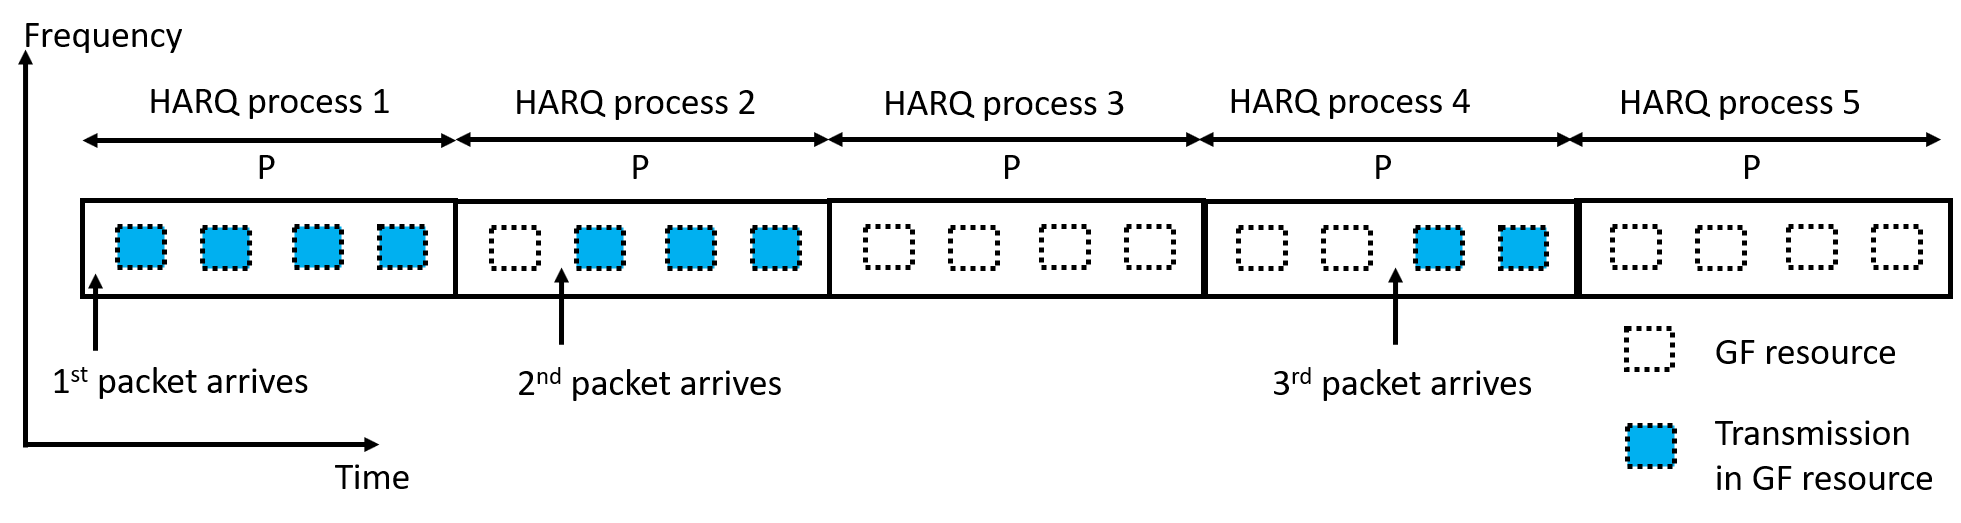
\includegraphics[scale=0.27]{fig1.png}}
\caption{Less than K repetitions in GF UL transmission.}
\label{fig1}
\end{figure}

Fig.~\ref{fig1} illustrates the situation when the number of configured repetitions is not ensured due to the constraint of boundary of period P. In Fig.~\ref{fig1}, an interval P contains 4 GF occasions, the UE is configured to do 4 repetitions. In the first period, data comes before all the 4 GF occasions so the UE is able to do 4 repetitions for the first packet as configured. However, when data comes in the second period, there are only 3 GF occasions left in that period. This means that the UE only can carry out 3 repetitions that are less than the configured number. Similarly, in the fourth period, the UE only can transmit the packet 2 times.

It is evident that when the packet comes after the first GF occasions in a period, the UE transmits the packet with a smaller number than the number configured by repK. It degrades the performance of uplink transmission. The situation becomes more severe for the URLLC UEs with high reliability requirement. Moreover, latency of a transmission also increases. After the gNB receives repetitions less than K repetitions, if it cannot decode the packet, it sends a retransmission request through an UL grant with HARQ ID of the process and NDI set to 0. The UE retransmits data on resources allocated by the gNB. Nevertheless, time consumption in this operation is high because the UE needs to wait the gNB to decode the packets and transmit an UL grant if necessary.

\subsection{Prior art}\label{ICC}
In 3GPP Release 15, the only option for the UE is to wait until the next period to start the transmission and fulfill the configured number of repetitions. Nevertheless, this option causes big delay and prevents the UE from meeting the URLLC latency requirement. 

In \cite{b1} and \cite{b2}, the repetitions are allowed to cross the boundary of a periodicity when the UE is not able to make the requiring repetitions. This solutions leads to a confusion of HARQ ID that makes the UE not be likely to differentiate the initial transmission and the retransmissions in order to combine and decode a specific codeblock. It has a huge impact on transmission reliability. Besides that, a new mechanism needs to be defined to communicate explicitly HARQ ID from the UE to the gNB and results in overhead and effort in standardization.  

Multiple configurations in GF region are proposed in \cite{b3} and \cite{b4}. A UE is configured with configurations having different time offsets so it can choose the nearest configuration to start a transmission and guarantee the number of repetitions. The main concern of multiple configurations is the control overhead because of signals used to configure the UE. The process to configure various configurations to the UE also causes delay. Moreover, if resources in the configurations are not overlapped, there will be an significant growth of resource consumption. In contrast, if the resources are overlapped, it might lead to a collision among transmissions of different UEs.

\cite{b5} and \cite{b7} propose to use shared resource for URLLC repetitions to improve resource utilization. However, they do not count a constraint that the UE cannot do repetitions crossing the border of a period. If this constraint is not solved, it might lead to a number of repetitions smaller than the  number configured and transmission reliability is degraded. In addition, shared resources are allocated periodically with the same size for all transmission occasions. These two drawbacks bring an increase of resource consumption and a drop of reliability 

In this work, an UL GF transmission scheme with reserved resources is described. Reserved resources are used and shared among the UEs when they need to transmit repetitions crossing the border of a transmission period P in order to achieve the target number of repetitions. These reserved resources have different sizes that are optimized based on the positions of their transmission occasions.  
Firstly, reserved resources and calculations to optimize their sizes are presented in Section \ref{II}. The process allowing the UEs to access to these resources is also discussed. Section \ref{III} shows numerical results obtaining from the equations derived in diverse scenarios. Finally, Section \ref{IV} provides the concluding remarks for this work.

\section{Improving reliability-latency by flexibly moving to explicit HARQ Feedback structure}\label{II}

\subsection{Operation of explicit HARQ feedback structure}\label{IIAA}

The HARQ structure in UL GF transmission is time-based. This means that there is no explicit ACK feedback sent from the gNB to the UE if data is decoded correctly. The UE uses a timer instead and waits until the end of time configured in the timer to determine a successful transmission if it does not receive an UL grant to schedule a retransmission. This structure has a drawback because the UE cannot differentiate between a successful transmission and miss-detection when the gNB cannot decode DMRS to identify the UE and transmits UL grant. Therefore, in case of miss-detection, the UE does not receive any signal from the gNB, it assumes a successful transmission and drops data in buffer. This behavior impacts reliability of a transmission and becomes more severe in less-than-K-repetitions situation. Once the UE is not able to carry the configured number of repetitions, the QoS of transmission is badly affected and there is a higher probability that the gNB cannot decode DMRS sequence. It leads to a degradation of URLLC transmission due to packet dropped by the UE. To handle the issue with GF transmissions with less than K repetitions, the transmission is proposed to use explicit HARQ feedback from the gNB. 

The transport block (TB) sent by the UE may result in three different scenarios, one for correct decoding, and two scenarios for incorrect decoding. In explicit HARQ feedback structure, the behavior of the UE in each scenario will be analyzed as follows. 

The first scenario is about correct data decoding. The gNB tries to combine all the repetitions of a transport block to facilitate data decoding, and the number of these repetitions can be less than K as per the previous discussion. For a normal operation, the base station receiver is capable of identifying the repetitions concerning a specific TB. Thus, whenever the base station is able to correctly decode a TB, and it sees that it was sent with less than K repetitions, it will send an explicit ACK for this TB to the transmitting UE.

The second scenario is about a failure of data decoding with a successful UE identification. When the UE transmits less than K repetitions, it’s possible that the data decoding is not successful but the base station is able to at least identify the user transmitting the TB with less than K repetitions. This can be feasible, for example, through identification of user specific DMRS sequence which it was configured with as part of CG configuration. In this case, the gNB will reschedule the UE for the re-transmission of the previously transmitted TB. 

The third scenario is related to failed UE identification. The bad quality of received data may lead to a situation when the base station is unable to identify the transmitting user. This situation is the most damaging for the URLLC UEs/applications due to their tight constraints on latency and reliability. With a timer based HARQ structure, which is currently used for URLLC transmissions in 3GPP Release 15, this situation leads to different understanding at the gNB and at the UE. The gNB, being unable to identify the UE, cannot schedule the re-transmission. The UE, upon receiving no UL grant for re-transmission, considers the packet successfully decoded at the gNB and discards the buffer upon the expiry of HARQ timer.

Although the situation when the gNB is not able to identify the user may be caused by a number of reasons such as the very bad channel conditions, large amount of interference or insufficient number of actual repetitions, to name but a few, the configuration parameters of CG transmission, in particular MCS and the number of repetitions K, are designed so as to combat most of these adverse effects. On the other hand, if the configured number of repetitions cannot be made, this brings the CG operation point to a lower QoS target than the desired operating point.

In the proposed technique, whenever the UE transmits less than K repetitions, the transport block in question is supposed to operate with explicit HARQ based feedback. In general, the gNB can identify transmissions with less than K repetitions thanks to DMRS detection and CG window boundary knowledge. When the gNB fails to identify the transmitting user and sends no ACK or UL grant to this UE, the UE upon expiry of configured HARQ timer re-transmits the TB. 

The re-transmission timing and resources can be configured as part of the explicit HARQ feedback configuration. One suitable option is to re-transmit in the closest CG periodic window after the expiry of HARQ feedback timer. The HARQ feedback timer should include the time for the gNB to decode the data and find the suitable occasion for potential DL transmission of HARQ ACK or UL grant.

\subsection{Design of explicit HARQ feedback}\label{IIBB}

In the proposed strategy, the UEs are allowed to request explicit-HARQ-feedback for certain transport blocks. Thus, a design for the explicit HARQ feedback in general may be needed. One strategy can be to define a channel where HARQ ACK/NAK can be transmitted. This can be similar to Physical HARQ Indicator Channel (PHICH) as specified in 4G LTE but this requires a lot of specification effort and high resource overhead. The rationale is that in typical operation mode, the users will not request explicit HARQ feedback and only in exceptional cases it will be required. 

With this in view, the proposal is to use the UL grant (DCI) as an explicit HARQ feedback. This DCI can be sent with user specific CS-RNTI which is used with configured GB transmissions. If the gNB is able to successfully decode the data, it can send an UL grant to this UE with the same HARQ process number (HARQ ID) as of the successfully received transport block, and the UE upon receiving this UL grant would know that this is in fact not a re-transmission request but an explicit ACK for the previously transmitted transport block. To avoid any confusion, new-data-indicator (NDI) field can be set to zero. Further, some of the fields in the DCI which are actually not needed, such as the time and frequency resource assignment fields, may be sent with fixed known values which can be pre-decided to be used in the ACK indication.

\section{Improving QoS (reliability-latency) by flexibly transmitting Scheduling Request }\label{III}

In this section, another scheme is proposed to deal with the problem of less-than-K repetitions. In this scheme to improve the reliability of UL GF transmissions, whenever the UE transmits less than the configured number of repetitions for a TB, it sends SR to the gNB, in parallel to transmission of TB with less than K repetitions.  This SR provides a sort of diversity mechanism in parallel to the transmission of the TB.

Release 15 does not allow transmission of PUCCH and PUSCH simultaneously. The UE transmits UCI encoding SR, HARQ feedback, etc on PUCCH. Therefore, the UE multiplexes UCI and PUSCH if it wants to transmit UCI while sending PUSCH. This strategy allows the UE to transmit SR that is UCI in case less than K repetitions are able to be carried out. However, a multiplexing of UCI and PUSCH deteriorate reliability and diversity of data on PUSCH and UCI. For this reason, SR should be configured to be transmitted on the configured PUCCH resources.

Table~\ref{tab1} shows in tabular format the UE and gNB actions for strategy of SR transmission in parallel to transmission of TB. 

\begin{table*}[htbp]
\caption{SR Transmission with TB and Actions for the gNB and the UE}
\begin{center}
\begin{tabular}{|p{1.5em}|p{9em}|p{9em}|p{12em}|p{9em}|p{9em}|}
 \hline
 \textbf{Case} & \textbf{GF PUSCH} & \textbf{SR in PUCCH} & \textbf{gNB understanding} & \textbf{gNB action} & \textbf{UE action}\\ 
 \hline
 1 & Correctly decoded at the gNB & Correctly decoded at the gNB & The gNB knows that SR is for the decoded TB & Indicate a correct detection (ex: using UL grant with the same HARQ ID) & Discard data upon receiving the gNB indication\\
 \hline
 2 &  Correctly decoded at the gNB & Incorrectly decoded at the gNB & The gNB upon correctly decoding the data and seeing less than K rep knows about missing SR. This case should be rare as SR is sent with strong coding & Indicate correct detection (ex: using UL grant with same HARQ ID) & Discard the data upon the gNB indication\\
\hline
3 & Incorrectly decoded at the gNB but UE Identified through DMRS & Correctly decoded at the gNB & the gNB understands that UE sent SR along with the TB that it failed to decoded & The gNB sends the UL grant for re-transmission & The UE follows the UL grant for re-transmission\\
\hline
4 & Incorrectly decoded and UE Identification Failure at the gNB & Correctly decoded at the gNB & The gNB completely misses the CG transmission due to failure in UE identification but it receives SR. From the timing of SR and CG configurations, the gNB knows its decoding failure & The gNB sends the UL grant for transmission & The UE follows the UL grant for transmission and re-transmits the data\\
\hline
5 & Incorrectly decoded at the gNB but UE Identified through DMRS & Incorrectly decoded at the gNB & The gNB identifies the UE from PUSCH. If it is able to identify the case of less than K repetitions, it knows also about SR detection failure & The gNB sends the UL grant for re-transmission & The UE follows the UL grant for re-transmission\\
\hline
 6 & Incorrectly decoded at the gNB and UE Identification Failure at the gNB & Incorrectly decoded at the gNB & The gNB has no indication about UE transmission & No action & The UE can be configured to
retransmit in the subsequent CG resources or SR\\
 

%  increase row height, number of & = number of collumn
% &&&&&\\[-1em]
 
 \hline
\end{tabular}
\label{tab1}
\end{center}
\end{table*}

The parallel transmission of PUCCH and PUSCH maybe slightly onerous for certain UEs but considering that the main focus is here on URLLC type of UEs with strict latency and reliability targets, this overhead may be acceptable.

In general, as Release-15 does not allow parallel transmission of PUCCH and PUSCH, the gNB upon receiving PUCCH and PUSCH from the same UE will understand that the SR in PUCCH is for the same TB sent in PUSCH for the UE that is only able to make less than K repetitions.

If the UE is transmitting different types of traffic at the same time, the gNB may get confused in making association of SR with the transmitted TB. In such a case, the proposed SR can be extended to differentiate from a standalone classic SR which is sent to the gNB to have the UL resources scheduled.  To do this, SR can comprise a field which indicates that this SR is for a TB being transmitted. Another strategy can be to indicate the HARQ ID of the transmitted TB in the SR. As upon receiving the TB, the base station will know its HARQ ID from its timing window, it will be able to conclude that the SR concerns the same TB or not.

Under certain situations, it may be beneficial to allow a hybrid scheme where the UEs can flexibly choose between an explicit HARQ feedback structure or sending an SR in parallel to the transmission of the transport block, when they are able to make less than K repetitions. The simplest scheme would be the one that the gNB configures the UEs to follow one of these two schemes. Alternatively, the UEs can be configured to choose one these two schemes. In that case, it would make sense to have an explicit indication in the TB for the explicit HARQ feedback. If the UEs choose to transmit SR in parallel to the transmission of the TB, they don’t trigger explicit feedback with the TB transmission. This can be advantageous in the situations when there is at least a suitable SR transmission occasion available where the UEs can transmit SR for the TB in question. In the contrary situation, the UEs don’t transmit SR in parallel to the transmission of the TB but send an indication to trigger explicit HARQ feedback. This can be more advantageous if for example, there is no suitable SR transmission occasion and a transmission of SR may harm the latency budget.

For the traffic with extremely stringent latency-reliability constraints, it can be foreseen that both mechanisms, explicit HARQ feedback and transmission of SR, are triggered in parallel to maximize the reliability within a short time interval when the UE has to transmit the TB with less than K repetitions.

\section{Conclusion}\label{IV}

In URLLC GF UL transmission. a packet is configured with K repetitions to achieve target QoS. However, because of boundary of a period P and arrival time of data, the UEs are only able to transmit less than K repetitions so the target QoS is not attained. This paper presents two strategies to help the UEs achieve the target QoS in case of less than K repetitions. These approaches relating to an explicit HARQ strucutre and an additional SR can be used individually or combined together based different scenarios.

\begin{thebibliography}{00}
\bibitem{b5} R. breu, G. Berardinelli, T. Jacobsen, K. Pedersen and P. Mogensen, ``A Blind Retransmission Scheme for Ultra-Reliable and Low Latency Communications'', 2018 IEEE 87th Vehicular Technology Conference (VTC Spring), June 2018.
\bibitem{b7} Z. Zhou, R. Ratasuk, N. Mangalvedhe and A. Ghosh, ``Resource Allocation for Uplink Grant-Free Ultra-Reliable and Low Latency Communications'', 2018 IEEE 87th Vehicular Technology Conference (VTC Spring), June 2018.
\bibitem{b9} B. Singh, O. Tirkkonen, Z. Li and M. A. Uusitalo, ``Contention-Based Access for Ultra-Reliable Low Latency Uplink Transmissions'',  IEEE Wireless Communications Letters, April 2018.
\bibitem{b1} Ericsson, ``Enhancement of Configured Grant for NR URLLC'', 3GPP R1-1812162, RAN1\#95, Spokane, USA, November 12--16, 2018.
\bibitem{b2} Huawei, HiSilicon, ``Enhanced UL configured grant transmissions'', 3GPP R1-1812226, RAN1\#95, Spokane, USA, November 12--16, 2018.
\bibitem{b3} Intel Corporation, ``On enhanced Configured Grant PUSCH for eURLLC'', 3GPP R1-1812506, RAN1\#95, Spokane, USA, November 12--16, 2018.
\bibitem{b4} Sony, ``Discussion on enhanced UL grant-free transmissions'', 3GPP R1-1812746, RAN1\#95, Spokane, USA, November 12--16, 2018.
\bibitem{b6} 3GPP TR 38.913 v15.0.0, ``Study on scenarios and requirements for next generation access technologies.''
\bibitem{b8} Huawei, HiSilicon, Nokia, Nokia Shanghai Bell, ``New SID on Physical Layer Enhancements for NR URLLC''. 3GPP RP-182089, TSG-RAN\#81, Gold Coast, Australia, Sept 10--13, 2018.
\bibitem{ad2} 3GPP TS 38.211 v15.3.0, ``Physical channels and modulation.''
\bibitem{ad3} 3GPP TR 38.802 v14.2.0, ``Study on new radio access technology physical layer aspects.''
\bibitem{ad4} 3GPP TS 38.214 v15.3.0, ``Physical layer procedures for data.''
\bibitem{ad5} 3GPP TS 38.331 v15.3.0, ``Radio Resource Control (RRC) protocol specification.''

\end{thebibliography}
\vspace{12pt}


\end{document}
